\documentclass{standalone}
\usepackage{tikz}
\usetikzlibrary{patterns, positioning}


\begin{document}
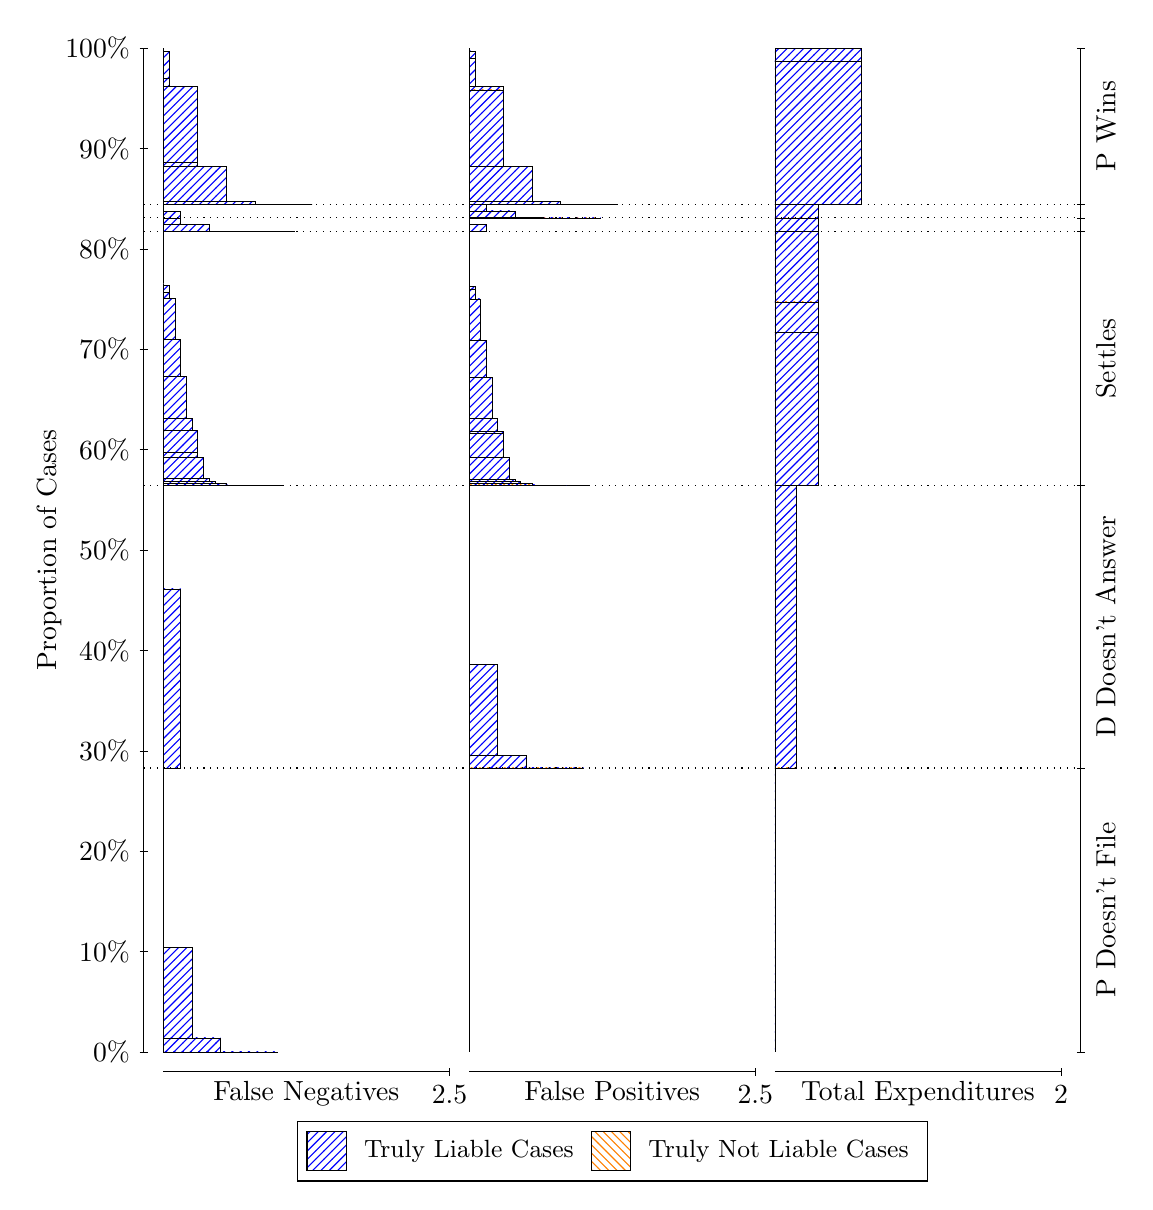
\begin{tikzpicture}
\draw[black, very thin] (1.5,1.75) -- (1.5,14.5);
\node[rotate=90, text=black, anchor=center] at (0.3, 8.125) {Proportion of Cases};
\draw[black, very thin] (1.45,1.75) -- (1.55,1.75);
\node[text=black, anchor=east] at (1.45, 1.75) {0\%};
\draw[black, very thin] (1.45,3.025) -- (1.55,3.025);
\node[text=black, anchor=east] at (1.45, 3.025) {10\%};
\draw[black, very thin] (1.45,4.3) -- (1.55,4.3);
\node[text=black, anchor=east] at (1.45, 4.3) {20\%};
\draw[black, very thin] (1.45,5.575) -- (1.55,5.575);
\node[text=black, anchor=east] at (1.45, 5.575) {30\%};
\draw[black, very thin] (1.45,6.85) -- (1.55,6.85);
\node[text=black, anchor=east] at (1.45, 6.85) {40\%};
\draw[black, very thin] (1.45,8.125) -- (1.55,8.125);
\node[text=black, anchor=east] at (1.45, 8.125) {50\%};
\draw[black, very thin] (1.45,9.4) -- (1.55,9.4);
\node[text=black, anchor=east] at (1.45, 9.4) {60\%};
\draw[black, very thin] (1.45,10.675) -- (1.55,10.675);
\node[text=black, anchor=east] at (1.45, 10.675) {70\%};
\draw[black, very thin] (1.45,11.95) -- (1.55,11.95);
\node[text=black, anchor=east] at (1.45, 11.95) {80\%};
\draw[black, very thin] (1.45,13.225) -- (1.55,13.225);
\node[text=black, anchor=east] at (1.45, 13.225) {90\%};
\draw[black, very thin] (1.45,14.5) -- (1.55,14.5);
\node[text=black, anchor=east] at (1.45, 14.5) {100\%};

\draw[black, very thin] (13.4,1.75) -- (13.4,14.5);
\draw[black, very thin] (13.35,1.75) -- (13.45,1.75);
\node[anchor=west] at (13.35, 1.75) {};
\draw[black, very thin] (13.35,5.3571) -- (13.45,5.3571);
\node[anchor=west] at (13.35, 5.3571) {};
\draw[black, very thin] (13.35,8.9451) -- (13.45,8.9451);
\node[anchor=west] at (13.35, 8.9451) {};
\draw[black, very thin] (13.35,12.173) -- (13.45,12.173);
\node[anchor=west] at (13.35, 12.173) {};
\draw[black, very thin] (13.35,12.344) -- (13.45,12.344);
\node[anchor=west] at (13.35, 12.344) {};
\draw[black, very thin] (13.35,12.515) -- (13.45,12.515);
\node[anchor=west] at (13.35, 12.515) {};
\draw[black, very thin] (13.35,14.5) -- (13.45,14.5);
\node[anchor=west] at (13.35, 14.5) {};

\draw[black, very thin, pattern color=blue, pattern=north east lines] (1.75,1.75) rectangle (3.2033,1.75);
\draw[black, very thin, pattern color=blue, pattern=north east lines] (1.75,1.75) rectangle (2.84,1.7515);
\draw[black, very thin, pattern color=blue, pattern=north east lines] (1.75,1.7515) rectangle (2.4767,1.9281);
\draw[black, very thin, pattern color=blue, pattern=north east lines] (1.75,1.9281) rectangle (2.1133,3.0821);
\draw[black, very thin, pattern color=orange, pattern=north west lines] (1.75,3.0821) rectangle (1.75,3.0821);
\draw[black, very thin, pattern color=blue, pattern=north east lines] (1.75,3.0821) rectangle (1.75,5.3571);
\draw[black, very thin, pattern color=blue, pattern=north east lines] (1.75,5.3571) rectangle (1.968,7.6324);
\draw[black, very thin, pattern color=orange, pattern=north west lines] (1.75,7.6324) rectangle (1.75,7.6324);
\draw[black, very thin, pattern color=blue, pattern=north east lines] (1.75,7.6324) rectangle (1.75,8.9451);
\draw[black, very thin, pattern color=blue, pattern=north east lines] (1.75,8.9451) rectangle (3.276,8.9451);
\draw[black, very thin, pattern color=blue, pattern=north east lines] (1.75,8.9451) rectangle (2.9853,8.9451);
\draw[black, very thin, pattern color=blue, pattern=north east lines] (1.75,8.9451) rectangle (2.9127,8.9451);
\draw[black, very thin, pattern color=blue, pattern=north east lines] (1.75,8.9451) rectangle (2.84,8.9451);
\draw[black, very thin, pattern color=blue, pattern=north east lines] (1.75,8.9451) rectangle (2.6947,8.9452);
\draw[black, very thin, pattern color=blue, pattern=north east lines] (1.75,8.9452) rectangle (2.622,8.9524);
\draw[black, very thin, pattern color=blue, pattern=north east lines] (1.75,8.9524) rectangle (2.5493,8.9681);
\draw[black, very thin, pattern color=blue, pattern=north east lines] (1.75,8.9681) rectangle (2.4767,8.9685);
\draw[black, very thin, pattern color=blue, pattern=north east lines] (1.75,8.9685) rectangle (2.404,8.9991);
\draw[black, very thin, pattern color=blue, pattern=north east lines] (1.75,8.9991) rectangle (2.3313,9.03);
\draw[black, very thin, pattern color=blue, pattern=north east lines] (1.75,9.03) rectangle (2.2587,9.3009);
\draw[black, very thin, pattern color=blue, pattern=north east lines] (1.75,9.3009) rectangle (2.186,9.3617);
\draw[black, very thin, pattern color=blue, pattern=north east lines] (1.75,9.3617) rectangle (2.186,9.6426);
\draw[black, very thin, pattern color=blue, pattern=north east lines] (1.75,9.6426) rectangle (2.1133,9.8031);
\draw[black, very thin, pattern color=blue, pattern=north east lines] (1.75,9.8031) rectangle (2.0407,10.332);
\draw[black, very thin, pattern color=blue, pattern=north east lines] (1.75,10.332) rectangle (1.968,10.798);
\draw[black, very thin, pattern color=blue, pattern=north east lines] (1.75,10.798) rectangle (1.8953,11.324);
\draw[black, very thin, pattern color=blue, pattern=north east lines] (1.75,11.324) rectangle (1.8227,11.393);
\draw[black, very thin, pattern color=blue, pattern=north east lines] (1.75,11.393) rectangle (1.8227,11.485);
\draw[black, very thin, pattern color=blue, pattern=north east lines] (1.75,11.485) rectangle (1.75,11.511);
\draw[black, very thin, pattern color=orange, pattern=north west lines] (1.75,11.511) rectangle (1.75,11.511);
\draw[black, very thin, pattern color=blue, pattern=north east lines] (1.75,11.511) rectangle (1.75,12.173);
\draw[black, very thin, pattern color=blue, pattern=north east lines] (1.75,12.173) rectangle (3.4213,12.173);
\draw[black, very thin, pattern color=blue, pattern=north east lines] (1.75,12.173) rectangle (3.058,12.173);
\draw[black, very thin, pattern color=blue, pattern=north east lines] (1.75,12.173) rectangle (2.6947,12.175);
\draw[black, very thin, pattern color=blue, pattern=north east lines] (1.75,12.175) rectangle (2.3313,12.261);
\draw[black, very thin, pattern color=blue, pattern=north east lines] (1.75,12.261) rectangle (1.968,12.344);
\draw[black, very thin, pattern color=orange, pattern=north west lines] (1.75,12.344) rectangle (1.75,12.344);
\draw[black, very thin, pattern color=blue, pattern=north east lines] (1.75,12.344) rectangle (1.968,12.427);
\draw[black, very thin, pattern color=orange, pattern=north west lines] (1.75,12.427) rectangle (1.75,12.427);
\draw[black, very thin, pattern color=blue, pattern=north east lines] (1.75,12.427) rectangle (1.75,12.515);
\draw[black, very thin, pattern color=blue, pattern=north east lines] (1.75,12.515) rectangle (3.6393,12.515);
\draw[black, very thin, pattern color=blue, pattern=north east lines] (1.75,12.515) rectangle (3.276,12.515);
\draw[black, very thin, pattern color=blue, pattern=north east lines] (1.75,12.515) rectangle (2.9127,12.55);
\draw[black, very thin, pattern color=blue, pattern=north east lines] (1.75,12.55) rectangle (2.5493,13);
\draw[black, very thin, pattern color=blue, pattern=north east lines] (1.75,13) rectangle (2.186,13.046);
\draw[black, very thin, pattern color=blue, pattern=north east lines] (1.75,13.046) rectangle (2.186,14.015);
\draw[black, very thin, pattern color=blue, pattern=north east lines] (1.75,14.015) rectangle (1.8227,14.11);
\draw[black, very thin, pattern color=blue, pattern=north east lines] (1.75,14.11) rectangle (1.8227,14.465);
\draw[black, very thin, pattern color=orange, pattern=north west lines] (1.75,14.465) rectangle (1.75,14.465);
\draw[black, very thin, pattern color=blue, pattern=north east lines] (1.75,14.465) rectangle (1.75,14.5);
\draw[black, very thin, pattern color=orange, pattern=north west lines] (5.6333,1.75) rectangle (5.6333,1.75);
\draw[black, very thin, pattern color=blue, pattern=north east lines] (5.6333,1.75) rectangle (5.6333,5.3571);
\draw[black, very thin, pattern color=orange, pattern=north west lines] (5.6333,5.3571) rectangle (7.0867,5.3571);
\draw[black, very thin, pattern color=blue, pattern=north east lines] (5.6333,5.3571) rectangle (7.0867,5.3571);
\draw[black, very thin, pattern color=blue, pattern=north east lines] (5.6333,5.3571) rectangle (6.7233,5.3576);
\draw[black, very thin, pattern color=blue, pattern=north east lines] (5.6333,5.3576) rectangle (6.36,5.5149);
\draw[black, very thin, pattern color=blue, pattern=north east lines] (5.6333,5.5149) rectangle (5.9967,6.6698);
\draw[black, very thin, pattern color=blue, pattern=north east lines] (5.6333,6.6698) rectangle (5.6333,8.9451);
\draw[black, very thin, pattern color=orange, pattern=north west lines] (5.6333,8.9451) rectangle (7.1593,8.9451);
\draw[black, very thin, pattern color=blue, pattern=north east lines] (5.6333,8.9451) rectangle (7.1593,8.9451);
\draw[black, very thin, pattern color=orange, pattern=north west lines] (5.6333,8.9451) rectangle (6.8687,8.9451);
\draw[black, very thin, pattern color=blue, pattern=north east lines] (5.6333,8.9451) rectangle (6.8687,8.9451);
\draw[black, very thin, pattern color=blue, pattern=north east lines] (5.6333,8.9451) rectangle (6.796,8.9451);
\draw[black, very thin, pattern color=orange, pattern=north west lines] (5.6333,8.9451) rectangle (6.7233,8.9451);
\draw[black, very thin, pattern color=blue, pattern=north east lines] (5.6333,8.9451) rectangle (6.7233,8.9451);
\draw[black, very thin, pattern color=orange, pattern=north west lines] (5.6333,8.9451) rectangle (6.578,8.9451);
\draw[black, very thin, pattern color=blue, pattern=north east lines] (5.6333,8.9451) rectangle (6.578,8.9451);
\draw[black, very thin, pattern color=blue, pattern=north east lines] (5.6333,8.9451) rectangle (6.5053,8.9523);
\draw[black, very thin, pattern color=orange, pattern=north west lines] (5.6333,8.9523) rectangle (6.4327,8.9523);
\draw[black, very thin, pattern color=blue, pattern=north east lines] (5.6333,8.9523) rectangle (6.4327,8.9676);
\draw[black, very thin, pattern color=orange, pattern=north west lines] (5.6333,8.9676) rectangle (6.4327,8.9676);
\draw[black, very thin, pattern color=blue, pattern=north east lines] (5.6333,8.9676) rectangle (6.4327,8.9677);
\draw[black, very thin, pattern color=blue, pattern=north east lines] (5.6333,8.9677) rectangle (6.36,8.9681);
\draw[black, very thin, pattern color=orange, pattern=north west lines] (5.6333,8.9681) rectangle (6.2873,8.9681);
\draw[black, very thin, pattern color=blue, pattern=north east lines] (5.6333,8.9681) rectangle (6.2873,8.9984);
\draw[black, very thin, pattern color=blue, pattern=north east lines] (5.6333,8.9984) rectangle (6.2147,9.0267);
\draw[black, very thin, pattern color=blue, pattern=north east lines] (5.6333,9.0267) rectangle (6.142,9.297);
\draw[black, very thin, pattern color=blue, pattern=north east lines] (5.6333,9.297) rectangle (6.0693,9.6067);
\draw[black, very thin, pattern color=blue, pattern=north east lines] (5.6333,9.6067) rectangle (6.0693,9.6331);
\draw[black, very thin, pattern color=orange, pattern=north west lines] (5.6333,9.6331) rectangle (5.9967,9.6331);
\draw[black, very thin, pattern color=blue, pattern=north east lines] (5.6333,9.6331) rectangle (5.9967,9.7945);
\draw[black, very thin, pattern color=blue, pattern=north east lines] (5.6333,9.7945) rectangle (5.924,10.32);
\draw[black, very thin, pattern color=blue, pattern=north east lines] (5.6333,10.32) rectangle (5.8513,10.786);
\draw[black, very thin, pattern color=blue, pattern=north east lines] (5.6333,10.786) rectangle (5.7787,11.315);
\draw[black, very thin, pattern color=blue, pattern=north east lines] (5.6333,11.315) rectangle (5.706,11.44);
\draw[black, very thin, pattern color=blue, pattern=north east lines] (5.6333,11.44) rectangle (5.706,11.476);
\draw[black, very thin, pattern color=blue, pattern=north east lines] (5.6333,11.476) rectangle (5.6333,12.173);
\draw[black, very thin, pattern color=orange, pattern=north west lines] (5.6333,12.173) rectangle (5.8513,12.173);
\draw[black, very thin, pattern color=blue, pattern=north east lines] (5.6333,12.173) rectangle (5.8513,12.256);
\draw[black, very thin, pattern color=blue, pattern=north east lines] (5.6333,12.256) rectangle (5.6333,12.344);
\draw[black, very thin, pattern color=orange, pattern=north west lines] (5.6333,12.344) rectangle (7.3047,12.344);
\draw[black, very thin, pattern color=blue, pattern=north east lines] (5.6333,12.344) rectangle (7.3047,12.344);
\draw[black, very thin, pattern color=blue, pattern=north east lines] (5.6333,12.344) rectangle (6.9413,12.344);
\draw[black, very thin, pattern color=blue, pattern=north east lines] (5.6333,12.344) rectangle (6.578,12.346);
\draw[black, very thin, pattern color=blue, pattern=north east lines] (5.6333,12.346) rectangle (6.2147,12.432);
\draw[black, very thin, pattern color=blue, pattern=north east lines] (5.6333,12.432) rectangle (5.8513,12.515);
\draw[black, very thin, pattern color=orange, pattern=north west lines] (5.6333,12.515) rectangle (7.5227,12.515);
\draw[black, very thin, pattern color=blue, pattern=north east lines] (5.6333,12.515) rectangle (7.5227,12.515);
\draw[black, very thin, pattern color=orange, pattern=north west lines] (5.6333,12.515) rectangle (7.1593,12.515);
\draw[black, very thin, pattern color=blue, pattern=north east lines] (5.6333,12.515) rectangle (7.1593,12.515);
\draw[black, very thin, pattern color=orange, pattern=north west lines] (5.6333,12.515) rectangle (6.796,12.515);
\draw[black, very thin, pattern color=blue, pattern=north east lines] (5.6333,12.515) rectangle (6.796,12.55);
\draw[black, very thin, pattern color=orange, pattern=north west lines] (5.6333,12.55) rectangle (6.4327,12.55);
\draw[black, very thin, pattern color=blue, pattern=north east lines] (5.6333,12.55) rectangle (6.4327,13);
\draw[black, very thin, pattern color=blue, pattern=north east lines] (5.6333,13) rectangle (6.0693,13.969);
\draw[black, very thin, pattern color=orange, pattern=north west lines] (5.6333,13.969) rectangle (6.0693,13.969);
\draw[black, very thin, pattern color=blue, pattern=north east lines] (5.6333,13.969) rectangle (6.0693,14.015);
\draw[black, very thin, pattern color=blue, pattern=north east lines] (5.6333,14.015) rectangle (5.706,14.37);
\draw[black, very thin, pattern color=blue, pattern=north east lines] (5.6333,14.37) rectangle (5.706,14.465);
\draw[black, very thin, pattern color=blue, pattern=north east lines] (5.6333,14.465) rectangle (5.6333,14.5);
\draw[black, very thin, pattern color=orange, pattern=north west lines] (9.5167,1.75) rectangle (9.5167,1.75);
\draw[black, very thin, pattern color=blue, pattern=north east lines] (9.5167,1.75) rectangle (9.5167,5.3571);
\draw[black, very thin, pattern color=orange, pattern=north west lines] (9.5167,5.3571) rectangle (9.7892,5.3571);
\draw[black, very thin, pattern color=blue, pattern=north east lines] (9.5167,5.3571) rectangle (9.7892,8.9451);
\draw[black, very thin, pattern color=orange, pattern=north west lines] (9.5167,8.9451) rectangle (10.062,8.9451);
\draw[black, very thin, pattern color=blue, pattern=north east lines] (9.5167,8.9451) rectangle (10.062,10.889);
\draw[black, very thin, pattern color=orange, pattern=north west lines] (9.5167,10.889) rectangle (10.062,10.889);
\draw[black, very thin, pattern color=blue, pattern=north east lines] (9.5167,10.889) rectangle (10.062,11.277);
\draw[black, very thin, pattern color=orange, pattern=north west lines] (9.5167,11.277) rectangle (10.062,11.277);
\draw[black, very thin, pattern color=blue, pattern=north east lines] (9.5167,11.277) rectangle (10.062,12.173);
\draw[black, very thin, pattern color=orange, pattern=north west lines] (9.5167,12.173) rectangle (10.062,12.173);
\draw[black, very thin, pattern color=blue, pattern=north east lines] (9.5167,12.173) rectangle (10.062,12.344);
\draw[black, very thin, pattern color=orange, pattern=north west lines] (9.5167,12.344) rectangle (10.062,12.344);
\draw[black, very thin, pattern color=blue, pattern=north east lines] (9.5167,12.344) rectangle (10.062,12.515);
\draw[black, very thin, pattern color=orange, pattern=north west lines] (9.5167,12.515) rectangle (10.607,12.515);
\draw[black, very thin, pattern color=blue, pattern=north east lines] (9.5167,12.515) rectangle (10.607,14.335);
\draw[black, very thin, pattern color=orange, pattern=north west lines] (9.5167,14.335) rectangle (10.607,14.335);
\draw[black, very thin, pattern color=blue, pattern=north east lines] (9.5167,14.335) rectangle (10.607,14.5);
\draw[black, dotted] (1.5,5.3571) -- (13.4,5.3571);
\draw[black, dotted] (1.5,8.9451) -- (13.4,8.9451);
\draw[black, dotted] (1.5,12.173) -- (13.4,12.173);
\draw[black, dotted] (1.5,12.344) -- (13.4,12.344);
\draw[black, dotted] (1.5,12.515) -- (13.4,12.515);
\draw[black, very thin] (1.75,1.5) -- (5.3833,1.5);
\node[text=black, anchor=north] at (3.5667, 1.5) {False Negatives};
\draw[black, very thin] (5.3833,1.45) -- (5.3833,1.55);
\node[text=black, anchor=north] at (5.3833, 1.45) {2.5};

\draw[black, very thin] (5.6333,1.5) -- (9.2667,1.5);
\node[text=black, anchor=north] at (7.45, 1.5) {False Positives};
\draw[black, very thin] (9.2667,1.45) -- (9.2667,1.55);
\node[text=black, anchor=north] at (9.2667, 1.45) {2.5};

\draw[black, very thin] (9.5167,1.5) -- (13.15,1.5);
\node[text=black, anchor=north] at (11.333, 1.5) {Total Expenditures};
\draw[black, very thin] (13.15,1.45) -- (13.15,1.55);
\node[text=black, anchor=north] at (13.15, 1.45) {2};

\node[text=black, centered, rotate=90] at (13.72, 3.5535) {P Doesn't File};
\node[text=black, centered, rotate=90] at (13.72, 7.1511) {D Doesn't Answer};
\node[text=black, centered, rotate=90] at (13.72, 10.559) {Settles};


\node[text=black, centered, rotate=90] at (13.72, 13.508) {P Wins};

\draw (7.449999999999999,1.5) node[draw=none] (baseCoordinate) {};
\begin{scope}[align=center]
        \matrix[scale=0.5, draw=black, below=0.5cm of baseCoordinate, nodes={draw}, column sep=0.1cm]{
            \node[rectangle, draw, minimum width=0.5cm, minimum height=0.5cm, pattern color=blue, pattern=north east lines] {}; &
            \node[draw=none, font=\small, text=black] (B) {Truly Liable Cases}; &
            \node[rectangle, draw, minimum width=0.5cm, minimum height=0.5cm, pattern color=orange, pattern=north west lines] {}; &
            \node[draw=none, font=\small, text=black] (B) {Truly Not Liable Cases}; \\
            };
\end{scope}

\end{tikzpicture}
\end{document}